\documentclass[aspectratio=43,11pt]{beamer}
\usetheme{default}
\usepackage[T1]{fontenc}
\usepackage{lmodern}
\usepackage{amsmath,amssymb,mathtools}
\usepackage{booktabs}
\usepackage{listings}
\usepackage{graphicx}
\usepackage{tikz}
\usepackage{pgfplots}
\pgfplotsset{compat=1.18}
\usetikzlibrary{arrows.meta,positioning,calc}
\graphicspath{{figures/}}
\definecolor{courseTeal}{RGB}{17,116,121}
\definecolor{courseBlue}{RGB}{25,60,85}
\definecolor{courseGrey}{RGB}{244,246,247}
\definecolor{courseOrange}{RGB}{206,111,36}
\definecolor{codeGrey}{RGB}{247,247,247}
\setbeamercolor{frametitle}{fg=courseBlue}
\setbeamerfont{frametitle}{series=\bfseries,size=\large}
\setbeamertemplate{navigation symbols}{}
\setbeamercolor{itemize item}{fg=courseTeal}
\setbeamercolor{itemize subitem}{fg=courseTeal}
\setbeamercolor{block title}{fg=white,bg=courseTeal}
\setbeamercolor{block body}{fg=black,bg=courseGrey}
\setbeamerfont{block title}{series=\bfseries,size=\small}
\setbeamerfont{block body}{size=\small}
\setbeamertemplate{blocks}[rounded][shadow=false]
\newcommand{\slideid}{L2}
\newcommand{\R}{\mathbb{R}}
\newcommand{\E}{\mathbb{E}}
\newenvironment{slideitems}{\small\begin{itemize}\setlength\itemsep{0.45em}}{\end{itemize}}
\newcommand{\tw}{0.47\textwidth}
\setbeamertemplate{footline}{\leavevmode\hbox{\begin{beamercolorbox}[wd=.70\paperwidth,ht=2.6ex,dp=1.0ex,leftskip=2em]{author in head/foot}\scriptsize Neural networks for supervised learning\end{beamercolorbox}\begin{beamercolorbox}[wd=.30\paperwidth,ht=2.6ex,dp=1.0ex,rightskip=2em plus1fil]{date in head/foot}\hfill\scriptsize \slideid\ -- \insertframenumber\end{beamercolorbox}}}
\lstset{basicstyle=\ttfamily\scriptsize,backgroundcolor=\color{codeGrey},frame=none,columns=fullflexible,keepspaces=true,showstringspaces=false,breaklines=true,escapeinside={(*@}{@*)}}
\title{Neural networks for supervised regression}
\subtitle{Chapter 2: Fundamentals of Machine Learning}
\begin{document}

\renewcommand{\slideid}{L2-S01}
\begin{frame}[t]{The supervised learning task}
\begin{slideitems}
\item We observe labelled examples $(x_i,y_i)$ and want a predictor $u_\theta$ that maps a new input $x$ to a plausible label.
\item Here we fit the model to input--output pairs. We will add PDE constraints in Chapter 3.
\item How well does $u_\theta$ predict data that were not used to fit $\theta$?
\end{slideitems}
\begin{center}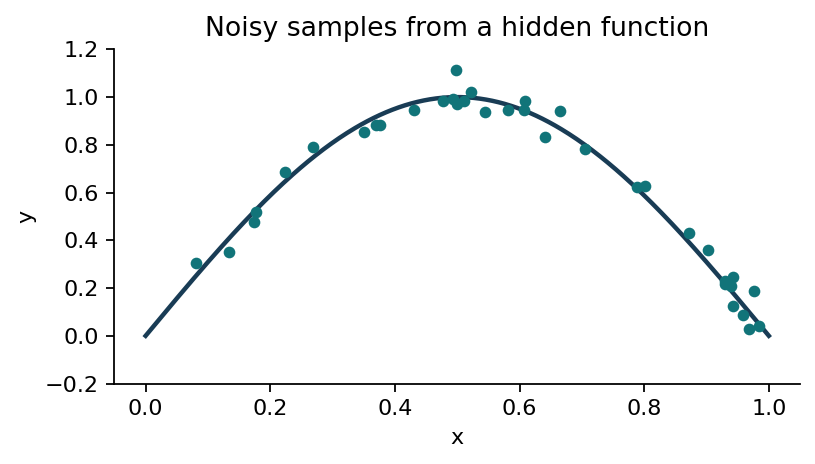
\includegraphics[height=3.1cm]{toy_data.png}\end{center}
\end{frame}

\renewcommand{\slideid}{L2-S02}
\begin{frame}[t]{Dataset notation and tensor shapes}
\begin{slideitems}
\item Store the inputs as rows and the labels as a column:
\[
X=\begin{bmatrix}x_1^\top\\ \vdots\\ x_N^\top\end{bmatrix}\in\R^{N\times d},\qquad
Y=\begin{bmatrix}y_1\\ \vdots\\ y_N\end{bmatrix}\in\R^{N\times 1}.
\]
\item For scalar regression, the network output should have the same shape:
\[
\widehat Y_\theta=u_\theta(X)=\begin{bmatrix}u_\theta(x_1)\\ \vdots\\ u_\theta(x_N)\end{bmatrix}\in\R^{N\times 1}.
\]
\item Check tensor shapes to catch silent broadcasting bugs, such as $(N,1)-(N,)$ becoming an $(N,N)$ matrix of residuals.
\end{slideitems}
\end{frame}

\renewcommand{\slideid}{L2-S03}
\begin{frame}[t]{Interpolation as a starting point}
\begin{slideitems}
\item Classical interpolation asks for exact agreement at prescribed points:
\[
p(x_i)=y_i,\qquad i=1,\ldots,N.
\]
\item Polynomial interpolation uses one global polynomial; piecewise-linear interpolation connects neighbours; cubic splines use smooth piecewise cubics.
\item For noisy data, we usually fit an average trend rather than require exact agreement at every point.
\end{slideitems}
\begin{center}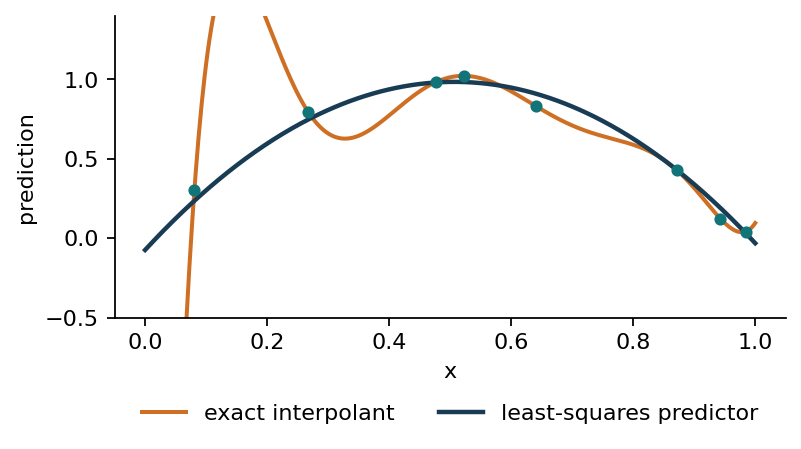
\includegraphics[height=2.75cm]{interp_vs_learning.png}\end{center}
\end{frame}

\renewcommand{\slideid}{L2-S04}
\begin{frame}[t]{Supervised regression is not interpolation}
\begin{slideitems}
\item Interpolation imposes constraints:
\[
u(x_i)=y_i\quad\text{for every observed point.}
\]
\item Regression minimises an average discrepancy:
\[
\min_\theta\; \frac1N\sum_{i=1}^N \bigl(u_\theta(x_i)-y_i\bigr)^2.
\]
\item With noisy labels, exact agreement can be undesirable. A predictor may generalise better by not passing through every sample.
\end{slideitems}
\begin{center}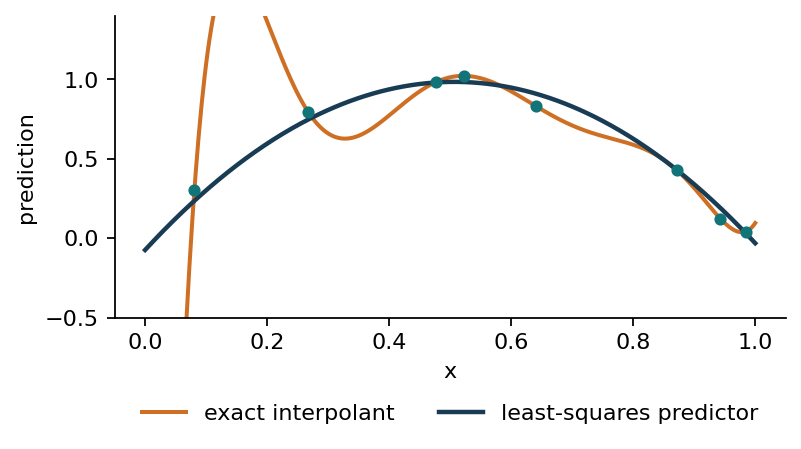
\includegraphics[height=2.65cm]{interp_vs_learning.png}\end{center}
\end{frame}

\renewcommand{\slideid}{L2-S05}
\begin{frame}[t]{The data-generating model}
\begin{slideitems}
\item A useful statistical model is
\[
Y=f_\star(X)+\varepsilon,\qquad \E[\varepsilon\mid X]=0.
\]
\item The unknown function $f_\star$ is the signal; $\varepsilon$ represents measurement noise or unresolved variability.
\item Training data are finite samples:
\[
\mathcal D_N=\{(x_i,y_i)\}_{i=1}^N\sim \rho^{\otimes N}.
\]
\item Generalisation means predicting new samples from the same distribution accurately.
\end{slideitems}
\end{frame}

\renewcommand{\slideid}{L2-S06}
\begin{frame}[t]{Population risk: the target quantity}
\begin{slideitems}
\item The ideal squared-loss risk is
\[
R(\theta)=\E_{(X,Y)\sim\rho}\Bigl[(u_\theta(X)-Y)^2\Bigr].
\]
\item If $Y=f_\star(X)+\varepsilon$ and $\E[\varepsilon\mid X]=0$, then
\[
R(\theta)=\|u_\theta-f_\star\|_{L^2(\rho_X)}^2 + \E[\varepsilon^2].
\]
\item The noise term is irreducible for this input. No deterministic model can remove it.
\end{slideitems}
\end{frame}

\renewcommand{\slideid}{L2-S07}
\begin{frame}[t]{Empirical risk: the computable quantity}
\begin{slideitems}
\item The population expectation is replaced by a finite average:
\[
R_N(\theta)=\frac1N\sum_{i=1}^N\bigl(u_\theta(x_i)-y_i\bigr)^2.
\]
\item Training means approximately solving
\[
\widehat\theta\approx \arg\min_{\theta\in\Theta} R_N(\theta).
\]
\item Training is approximate: we stop after finitely many updates and may not find a global minimum. The finite-data loss also differs from population risk.
\end{slideitems}
\end{frame}

\renewcommand{\slideid}{L2-S08}
\begin{frame}[fragile,t]{Generating a toy dataset in code}
\begin{columns}[T,totalwidth=\textwidth]
\begin{column}{0.51\textwidth}
\begin{slideitems}
\item A simple regression test case is noisy data from a smooth target.
\item Fix the data and random seed before comparing models.
\end{slideitems}
\begin{lstlisting}
rng = np.random.default_rng(4)
x = np.sort(rng.uniform(0, 1, 64))[:, None]
y_clean = np.sin(np.pi * x)
y = y_clean + 0.05 * rng.normal(size=x.shape)
\end{lstlisting}
\end{column}
\begin{column}{0.45\textwidth}
\centering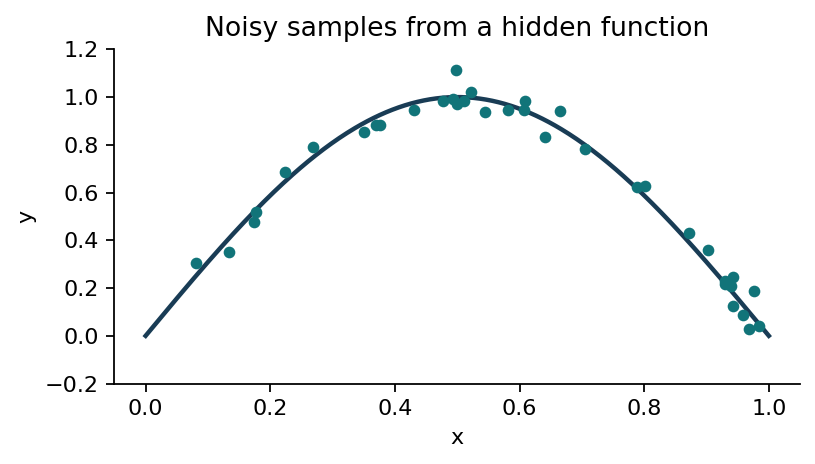
\includegraphics[width=\linewidth]{toy_data.png}
\end{column}
\end{columns}
\end{frame}

\renewcommand{\slideid}{L2-S09}
\begin{frame}[t]{What the plot tells us before training}
\begin{slideitems}
\item The samples suggest a smooth one-dimensional pattern, but the labels are not exactly on the hidden curve.
\item A model that follows every noisy point may have low training error and higher prediction error.
\item A model that is too rigid may miss the curvature even if it is stable.
\end{slideitems}
\begin{center}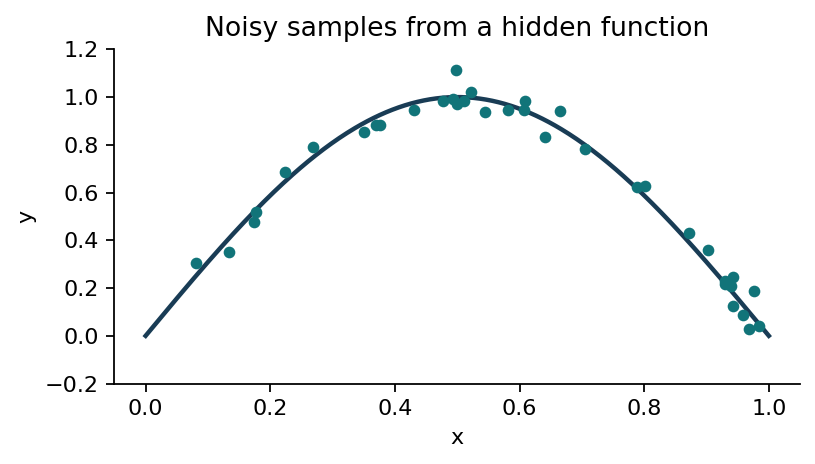
\includegraphics[height=3.15cm]{toy_data.png}\end{center}
\end{frame}

\renewcommand{\slideid}{L2-S10}
\begin{frame}[t]{Start with an affine baseline}
\begin{slideitems}
\item The simplest model is
\[
u_{w,b}(x)=wx+b.
\]
\item The residuals are
\[
r_i=wx_i+b-y_i.
\]
\item The training objective is a convex quadratic:
\[
L(w,b)=\frac1N\sum_{i=1}^N r_i^2.
\]
\item We can solve this problem directly, then see how much error comes from fitting a straight line.
\end{slideitems}
\end{frame}

\renewcommand{\slideid}{L2-S11}
\begin{frame}[t]{Linear regression in matrix form}
\begin{slideitems}
\item Introduce the design matrix
\[
A=\begin{bmatrix}x_1&1\\ \vdots&\vdots\\ x_N&1\end{bmatrix},\qquad \beta=\begin{bmatrix}w\\b\end{bmatrix}.
\]
\item The fitted values are $A\beta$ and the empirical loss is
\[
L(\beta)=\frac1N\|A\beta-Y\|_2^2.
\]
\item The gradient is
\[
\nabla_\beta L(\beta)=\frac{2}{N}A^\top(A\beta-Y).
\]
\end{slideitems}
\end{frame}

\renewcommand{\slideid}{L2-S12}
\begin{frame}[t]{The normal equations}
\begin{slideitems}
\item Setting the gradient to zero gives
\[
A^\top A\,\widehat\beta=A^\top Y.
\]
\item If $A^\top A$ is nonsingular, then
\[
\widehat\beta=(A^\top A)^{-1}A^\top Y.
\]
\item In practice, a least-squares solver is more stable than explicitly forming the inverse.
\item Here we can find a global minimiser by solving a linear system.
\end{slideitems}
\end{frame}

\renewcommand{\slideid}{L2-S13}
\begin{frame}[fragile,t]{The baseline in NumPy}
\begin{slideitems}
\item The two-column matrix stores the slope feature and the intercept feature.
\end{slideitems}
\begin{lstlisting}
A = np.column_stack([train_x[:, 0], np.ones(len(train_x))])
beta, *_ = np.linalg.lstsq(A, train_y[:, 0], rcond=None)
w, b = beta
prediction = w * test_x[:, 0] + b
mse = np.mean((prediction - test_y[:, 0])**2)
\end{lstlisting}
\begin{slideitems}
\item The optimisation error is essentially zero; any remaining error is due to model rigidity and finite data.
\end{slideitems}
\end{frame}

\renewcommand{\slideid}{L2-S14}
\begin{frame}[t]{What the affine baseline cannot express}
\begin{slideitems}
\item A straight line has no curvature:
\[
\frac{d^2}{dx^2}(wx+b)=0.
\]
\item The hidden target $\sin(\pi x)$ has curvature:
\[
\frac{d^2}{dx^2}\sin(\pi x)=-\pi^2\sin(\pi x).
\]
\item Even the best straight line will miss this curvature.
\end{slideitems}
\begin{center}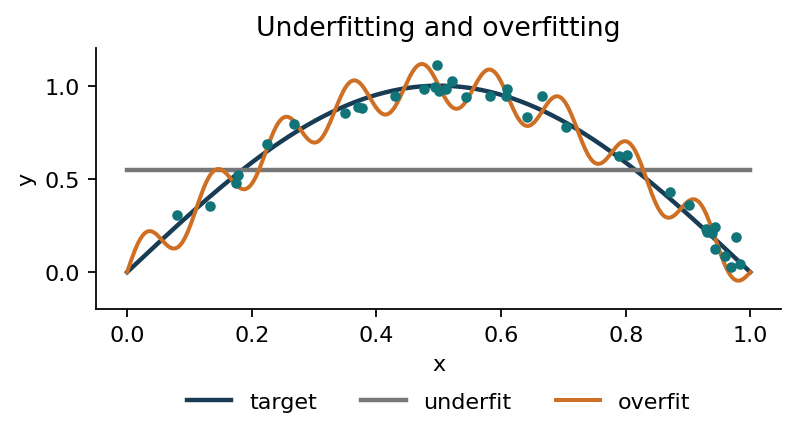
\includegraphics[height=2.8cm]{under_over.png}\end{center}
\end{frame}

\renewcommand{\slideid}{L2-S15}
\begin{frame}[t]{A neural network as nested functions}
\begin{slideitems}
\item A two-hidden-layer scalar network can be written as
\[
a^{(1)}=\sigma(W_1x+b_1),\qquad a^{(2)}=\sigma(W_2a^{(1)}+b_2),
\]
\[
u_\theta(x)=W_3a^{(2)}+b_3.
\]
\item The parameter vector is
\[
\theta=(W_1,b_1,W_2,b_2,W_3,b_3).
\]
\item Training chooses the weights and biases from data; the architecture specifies the allowed compositions.
\end{slideitems}
\end{frame}


\renewcommand{\slideid}{L2-S16}
\begin{frame}[t]{Why call it a neural network?}
\begin{slideitems}
\item The name comes from an analogy with biological neural systems: many simple units send signals along connections.
\item In the artificial model, the unit is much simpler: it computes a weighted sum, adds a bias, and applies a scalar nonlinearity.
\item The biological analogy explains the name. Mathematically, we compose parametrised functions.
\end{slideitems}
\begin{center}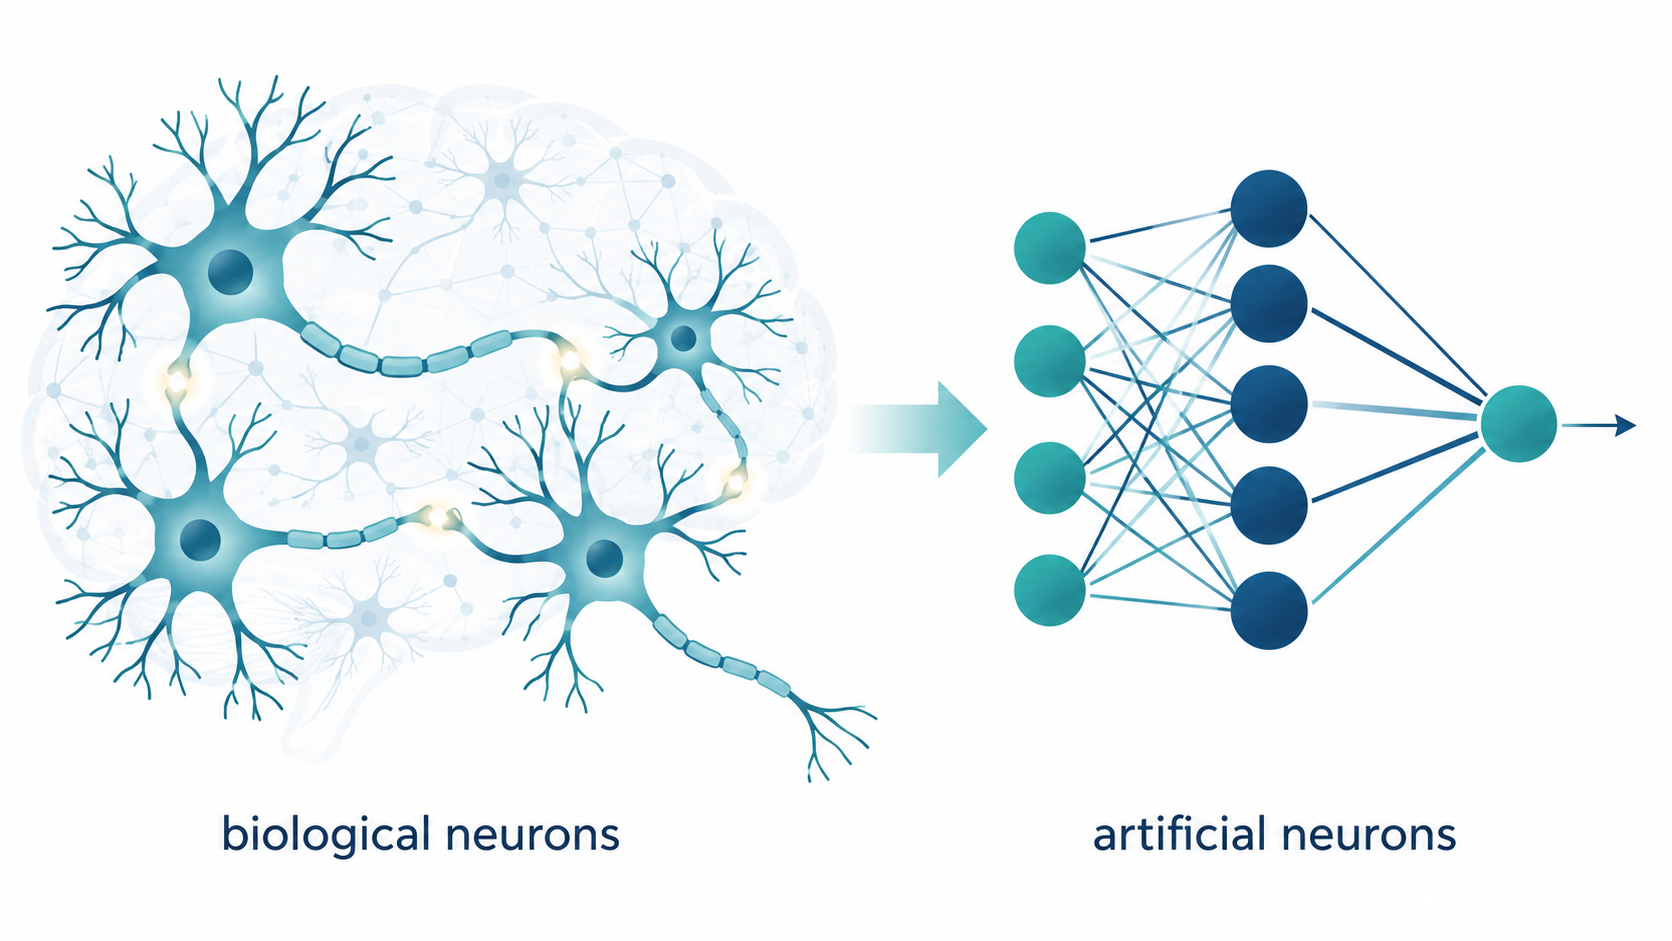
\includegraphics[height=3.05cm]{brain_to_ann.png}\end{center}
\end{frame}

\renewcommand{\slideid}{L2-S17}
\begin{frame}[t]{From a biological neuron to an artificial one}
\begin{slideitems}
\item A biological neuron receives many inputs through dendrites and sends an output signal along an axon.
\item An artificial neuron receives numbers $x_1,\ldots,x_d$ and computes one number:
\[
 z=w\cdot x+b=\sum_{j=1}^d w_jx_j+b,\qquad a=\sigma(z).
\]
\item Weights play the role of connection strengths. The activation $\sigma$ is a simple firing rule, not a realistic model of cell biology.
\item A layer repeats this computation in parallel.
\end{slideitems}
\end{frame}

\renewcommand{\slideid}{L2-S18}
\begin{frame}[t]{One artificial neuron}
\begin{columns}[T,totalwidth=\textwidth]
\begin{column}{0.48\textwidth}
\begin{slideitems}
\item A single neuron has parameters $(w,b)$ and output
\[
 x\longmapsto \sigma(w\cdot x+b).
\]
\item The hyperplane $w\cdot x+b=0$ is the transition region of the neuron.
\item Larger $\|w\|$ makes the transition sharper; changing $b$ shifts it.
\end{slideitems}
\end{column}
\begin{column}{0.48\textwidth}
\centering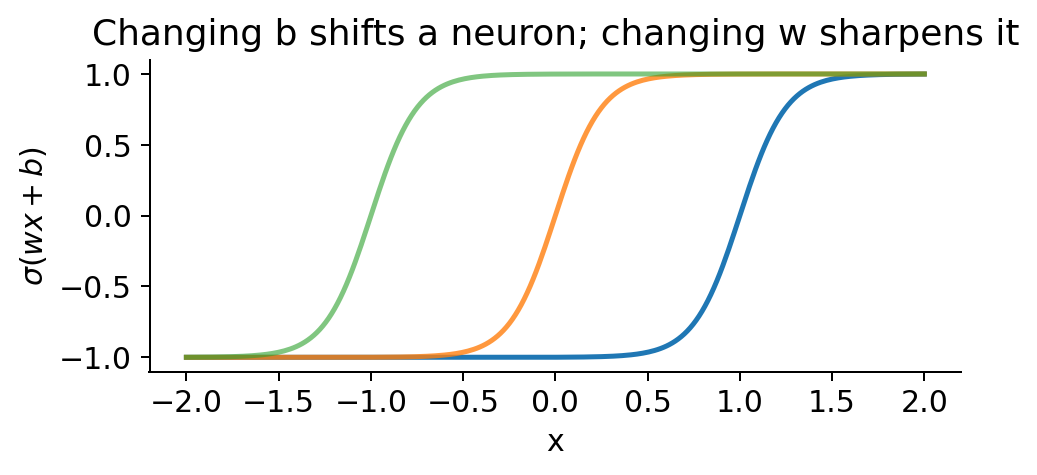
\includegraphics[width=\linewidth]{shifted_neurons.png}
\end{column}
\end{columns}
\end{frame}

\renewcommand{\slideid}{L2-S19}
\begin{frame}[t]{A layer as parallel neurons}
\begin{slideitems}
\item A layer with $m$ neurons computes
\[
 a(x)=\sigma(Wx+b)\in\mathbb R^m,
\]
where $W\in\mathbb R^{m\times d}$ and $b\in\mathbb R^m$.
\item Componentwise, this is
\[
 a_j(x)=\sigma(w_j\cdot x+b_j),\qquad j=1,\ldots,m.
\]
\item The layer turns the input into $m$ learned features. The next layer combines those features.
\end{slideitems}
\begin{center}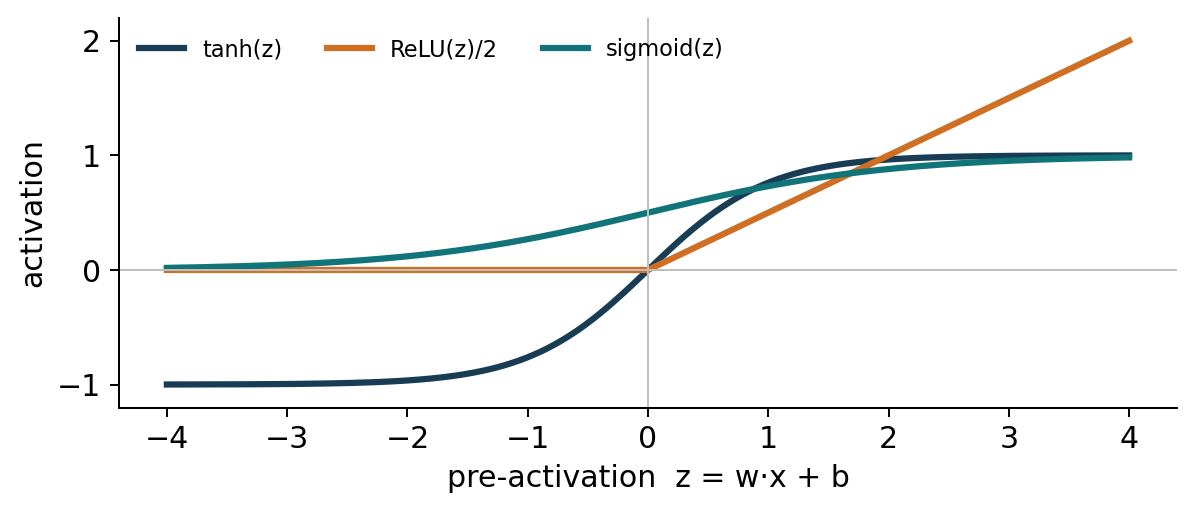
\includegraphics[height=2.2cm]{activation_functions.png}\end{center}
\end{frame}

\renewcommand{\slideid}{L2-S20}
\begin{frame}[t]{A shallow network}
\begin{slideitems}
\item A one-hidden-layer network has the form
\[
 u_n(x)=c_0+\sum_{j=1}^n c_j\,\sigma(w_j\cdot x+b_j).
\]
\item The inner parameters $(w_j,b_j)$ choose the features. The outer coefficients $c_j$ combine them.
\item The approximation family is
\[
 \mathcal M_n(\sigma)=\left\{c_0+\sum_{j=1}^n c_j\sigma(w_j\cdot x+b_j)\right\}.
\]
\item Universal approximation asks whether $\bigcup_n\mathcal M_n(\sigma)$ is dense in a function space.
\end{slideitems}
\end{frame}

\renewcommand{\slideid}{L2-S21}
\begin{frame}[t]{What universal approximation means}
\begin{slideitems}
\item A density statement has the form
\[
 \forall f\in C(K),\quad \forall \varepsilon>0,
 \quad \exists n,\exists u_n\in\mathcal M_n(\sigma):
 \|f-u_n\|_{\infty,K}<\varepsilon.
\]
\item This is an existence theorem. It says the family contains a good approximant.
\item It does not say how large $n$ must be, how large the weights are, or whether gradient-based training will find the approximant.
\end{slideitems}
\begin{center}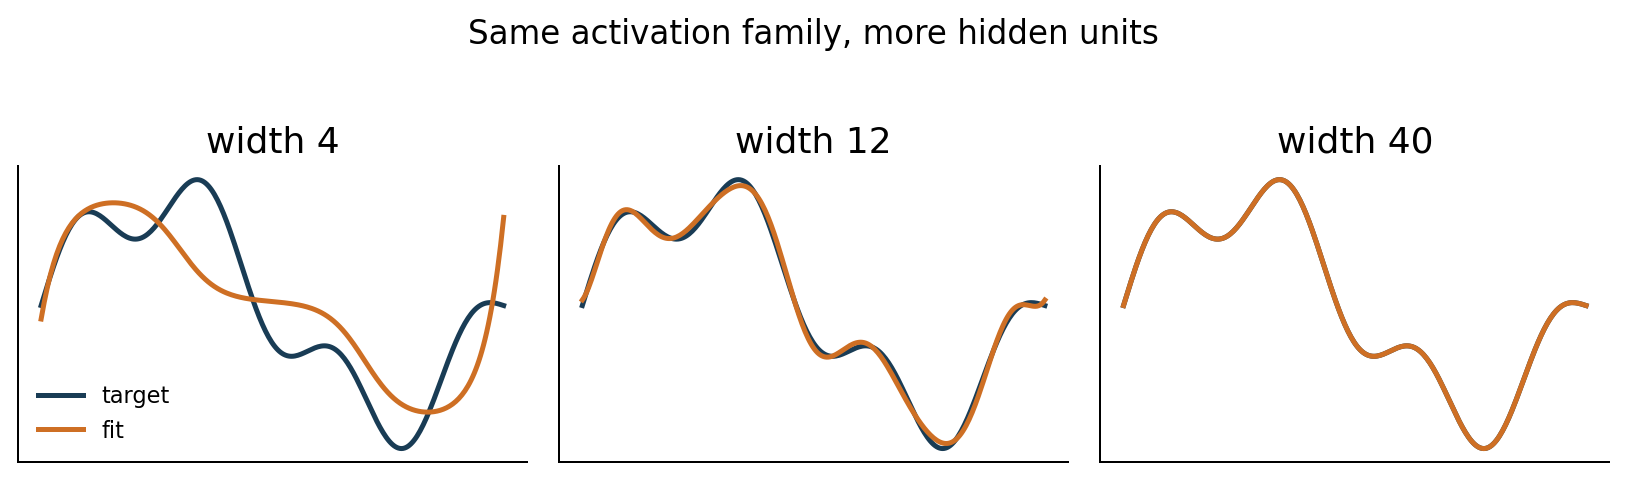
\includegraphics[height=2.35cm]{uat_width_demo.png}\end{center}
\end{frame}

\renewcommand{\slideid}{L2-S22}
\begin{frame}[t]{Cybenko's universal approximation theorem}
\begin{block}{Theorem (Cybenko, 1989)}
Let $\sigma:\mathbb R\to\mathbb R$ be continuous and sigmoidal, meaning
\[
 \lim_{t\to-\infty}\sigma(t)=0,
 \qquad
 \lim_{t\to+\infty}\sigma(t)=1.
\]
Then finite sums
\[
 \sum_{j=1}^n c_j\sigma(w_j\cdot x+b_j)
\]
are dense in $C([0,1]^d)$ in the uniform norm.
\end{block}
\begin{slideitems}
\item The width may grow with the target function and the requested accuracy.
\end{slideitems}
\end{frame}

\renewcommand{\slideid}{L2-S23}
\begin{frame}[t]{Cybenko proof sketch: separate by a functional}
\begin{slideitems}
\item Let $S$ be the uniform closure of all finite sums of neurons.
\item Suppose, for contradiction, that $S\ne C([0,1]^d)$.
\item By Hahn--Banach, there is a nonzero continuous linear functional $L$ such that
\[
 L(g)=0\quad\text{for every }g\in S.
\]
\item By the Riesz representation theorem, there is a nonzero signed measure $\mu$ with
\[
 L(g)=\int_{[0,1]^d} g(x)\,d\mu(x).
\]
\end{slideitems}
\end{frame}

\renewcommand{\slideid}{L2-S24}
\begin{frame}[t]{Cybenko proof sketch: annihilating neurons}
\begin{slideitems}
\item Since every neuron lies in $S$, the measure satisfies
\[
 \int_{[0,1]^d}\sigma(w\cdot x+b)\,d\mu(x)=0
 \qquad\text{for all } w,b.
\]
\item The sigmoidal property lets scaled neurons approximate half-space indicators:
\[
 \sigma\bigl(\lambda(w\cdot x+b)\bigr)
 \longrightarrow \mathbf 1_{\{w\cdot x+b>0\}}
 \quad\text{as }\lambda\to\infty.
\]
\item Passing to the limit shows that $\mu$ assigns zero mass to all half-spaces.
\end{slideitems}
\end{frame}

\renewcommand{\slideid}{L2-S25}
\begin{frame}[t]{Cybenko proof sketch: the contradiction}
\begin{slideitems}
\item If a finite signed measure vanishes on all half-spaces, then it is the zero measure.
\item One way to see the last step is through Fourier analysis: half-space information determines the Fourier transform of the measure.
\item Thus $\mu=0$, contradicting the nonzero measure supplied by Hahn--Banach.
\item Therefore the closure $S$ must be the whole space $C([0,1]^d)$.
\end{slideitems}
\end{frame}

\renewcommand{\slideid}{L2-S26}
\begin{frame}[t]{The Pinkus / LLPS sharpening}
\begin{block}{Theorem (Leshno--Lin--Pinkus--Schocken, 1993)}
For continuous $\sigma$, the family of one-hidden-layer networks is dense in $C(K)$ for every compact $K\subset\mathbb R^d$ if and only if $\sigma$ is not a polynomial.
\end{block}
\begin{slideitems}
\item The activation can be any continuous non-polynomial function; it need not be sigmoidal.
\item ReLU, tanh, sigmoid, softplus and many other non-polynomial activations satisfy the density condition.
\end{slideitems}
\end{frame}

\renewcommand{\slideid}{L2-S27}
\begin{frame}[t]{Why polynomials are the obstruction}
\begin{slideitems}
\item If $\sigma$ is a polynomial of degree $m$, then every neuron $\sigma(w\cdot x+b)$ is also a polynomial of degree at most $m$.
\item Finite sums remain in the same finite-dimensional polynomial space.
\item A finite-dimensional proper subspace of $C(K)$ is closed and cannot be dense.
\item Thus a polynomial activation cannot be universal.
\end{slideitems}
\end{frame}

\renewcommand{\slideid}{L2-S28}
\begin{frame}[t]{Pinkus proof sketch I: stay inside the span}
\begin{slideitems}
\item In one dimension, consider the dictionary functions $x\mapsto\sigma(wx+b)$.
\item Difference quotients in the inner weight remain in the span before taking the limit:
\[
 \frac{\sigma((w+h)x+b)-\sigma(wx+b)}{h}.
\]
\item If $\sigma$ is smooth, the limit gives
\[
 x\,\sigma'(wx+b)\in\overline{\mathrm{span}\{\sigma(wx+b)\}}.
\]
\item Iterating the argument produces
\[
 x^k\sigma^{(k)}(wx+b)\quad\text{in the closure.}
\]
\end{slideitems}
\end{frame}

\renewcommand{\slideid}{L2-S29}
\begin{frame}[t]{Pinkus proof sketch II: recover monomials}
\begin{slideitems}
\item Set $w=0$ in the previous expression:
\[
 x^k\sigma^{(k)}(b)\in \overline{\mathrm{span}}.
\]
\item If $\sigma$ is not a polynomial, then for every $k$ there is some $b_k$ with
\[
 \sigma^{(k)}(b_k)\ne 0.
\]
\item Hence each monomial $x^k$ lies in the closure of the network span.
\item Since polynomials are dense in $C(K)$ by Weierstrass, the network span is dense.
\end{slideitems}
\end{frame}

\renewcommand{\slideid}{L2-S30}
\begin{frame}[t]{Pinkus proof sketch III: remove smoothness}
\begin{slideitems}
\item The previous argument was written for smooth $\sigma$ to show the mechanism.
\item For merely continuous activations, convolve with a smooth mollifier:
\[
 \sigma_\delta=\sigma*\varphi_\delta.
\]
\item Translates of $\sigma_\delta$ are limits of finite sums of translates of $\sigma$, so the smoothed activation remains in the closure generated by $\sigma$.
\item Apply the smooth argument to a non-polynomial mollification and then pass back to $\sigma$.
\end{slideitems}
\end{frame}

\renewcommand{\slideid}{L2-S31}
\begin{frame}[t]{What remains after an approximation theorem}
\begin{slideitems}
\item We still need an algorithm to find the weights.
\item We need a practical width for the requested accuracy.
\item The weights may be large.
\item Error on the training data can differ from population risk.
\item Optimisation and generalisation need separate analysis.
\end{slideitems}
\end{frame}

\renewcommand{\slideid}{L2-S32}
\begin{frame}[t]{Universal approximation in a toy plot}
\begin{slideitems}
\item Increasing the number of hidden units gives a larger function family.
\item In this least-squares example, adding hidden units makes the fitted curve more flexible.
\item The theorem explains why approximation is possible in principle; the experiment still depends on feature placement, conditioning, and optimisation.
\end{slideitems}
\begin{center}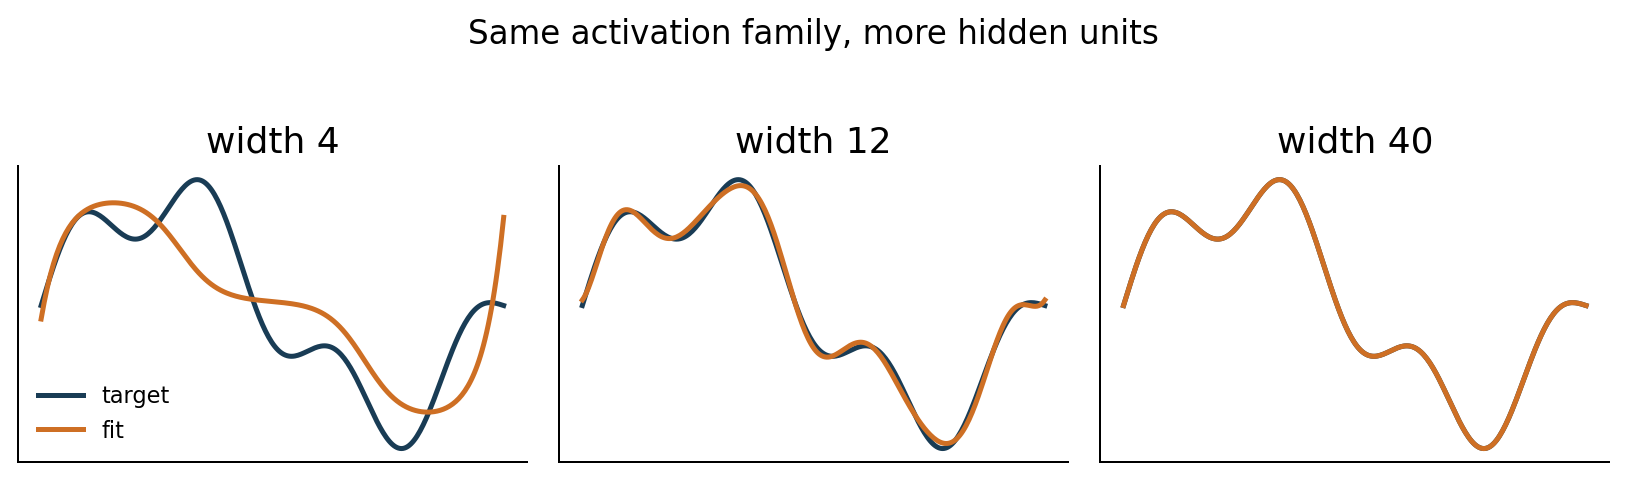
\includegraphics[height=2.8cm]{uat_width_demo.png}\end{center}
\end{frame}

\renewcommand{\slideid}{L2-S33}
\begin{frame}[t]{From approximation to training}
\begin{slideitems}
\item The theorems justify using neural-network families as flexible approximators.
\item Next we work through training and evaluation:
\[
 \text{data} \rightarrow \text{empirical loss} \rightarrow \text{optimiser} \rightarrow \text{validation/test error}.
\]
\item There are three sources of error to consider: approximation, optimisation, and estimation.
\item Universal approximation addresses only the first one.
\end{slideitems}
\end{frame}


\renewcommand{\slideid}{L2-S34}
\begin{frame}[t]{One hidden layer is enough for density}
\begin{slideitems}
\item The universal approximation theorems already apply to shallow networks:
\[
 u_n(x)=c_0+\sum_{j=1}^n c_j\sigma(w_j\cdot x+b_j).
\]
\item Depth is not needed to obtain density in $C(K)$.
\item Depth can still matter for efficiency: some compositional functions may need fewer parameters when represented by deeper architectures.
\item Density alone leaves open the required model size, training cost, and amount of data.
\end{slideitems}
\end{frame}

\renewcommand{\slideid}{L2-S35}
\begin{frame}[t]{Why existence does not settle training}
\begin{slideitems}
\item The theorem states existence:
\[
 \inf_{u\in\mathcal M_n}\|f-u\|\to 0.
\]
\item Training solves a different finite-data problem:
\[
 \widehat\theta \approx \arg\min_\theta \frac1N\sum_{i=1}^N (u_\theta(x_i)-y_i)^2.
\]
\item To find a useful fit from finite data, we also need optimisation, regularisation, and independent evaluation.
\end{slideitems}
\end{frame}

\renewcommand{\slideid}{L2-S36}
\begin{frame}[t]{Shape bookkeeping for a width-32 MLP}
\begin{slideitems}
\item With batch size $N$ and scalar input, the tensors have shapes
\[
X:(N,1),\quad A^{(1)}:(N,32),\quad A^{(2)}:(N,32),\quad U_\theta:(N,1).
\]
\item The matrix dimensions are
\[
W_1:(1,32),\quad W_2:(32,32),\quad W_3:(32,1),
\]
using the common row-sample convention.
\item Check these dimensions before computing the loss.
\end{slideitems}
\end{frame}

\renewcommand{\slideid}{L2-S37}
\begin{frame}[t]{Width and depth as modelling choices}
\begin{slideitems}
\item Width increases the number of hidden features available at a given layer.
\item Depth increases the number of nonlinear compositions.
\item More width or depth can reduce approximation error, but it can also increase estimation difficulty and optimisation sensitivity.
\item Compare models using the same data splits and training budget, then check validation error.
\end{slideitems}
\begin{center}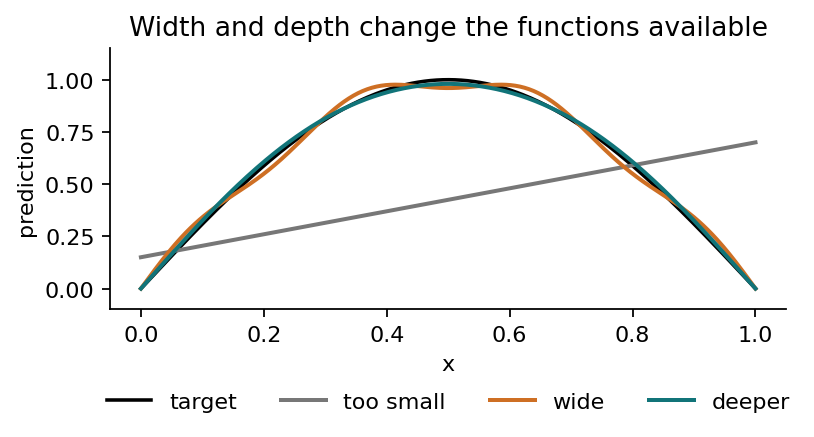
\includegraphics[height=2.75cm]{width_depth_predictions.png}\end{center}
\end{frame}

\renewcommand{\slideid}{L2-S38}
\begin{frame}[t]{Counting parameters}
\begin{slideitems}
\item For a network $1\to 32\to 32\to 1$, the parameter count is
\[
(1\cdot 32+32)+(32\cdot 32+32)+(32\cdot 1+1).
\]
\item Therefore
\[
64+1056+33=1153.
\]
\item Record the parameter count when comparing models; accuracy also depends on training and data.
\item With only tens of training points, the model can be much larger than the dataset.
\end{slideitems}
\end{frame}

\renewcommand{\slideid}{L2-S39}
\begin{frame}[fragile,t]{The PyTorch model}
\begin{slideitems}
\item The model definition states the architecture, activation, and numerical dtype.
\end{slideitems}
\begin{lstlisting}
model = torch.nn.Sequential(
    torch.nn.Linear(1, 32, dtype=torch.float64),
    torch.nn.Tanh(),
    torch.nn.Linear(32, 32, dtype=torch.float64),
    torch.nn.Tanh(),
    torch.nn.Linear(32, 1, dtype=torch.float64),
)
assert sum(p.numel() for p in model.parameters()) == 1153
\end{lstlisting}
\begin{slideitems}
\item The final layer is linear because this is scalar regression, not classification.
\end{slideitems}
\end{frame}

\renewcommand{\slideid}{L2-S40}
\begin{frame}[t]{Why an activation is necessary}
\begin{slideitems}
\item A composition of affine maps is affine:
\[
W_2(W_1x+b_1)+b_2=(W_2W_1)x+(W_2b_1+b_2).
\]
\item Without a nonlinear activation, depth would not create a nonlinear predictor.
\item A nonlinear activation lets the network represent curved functions.
\end{slideitems}
\begin{center}
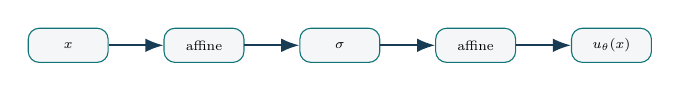
\begin{tikzpicture}[scale=0.70, transform shape, every node/.style={font=\scriptsize}, box/.style={draw=courseTeal,rounded corners,align=center,minimum width=1.45cm,minimum height=.62cm,fill=courseGrey}, arr/.style={-Latex,thick,courseBlue}]
\node[box] (x) {$x$};\node[box,right=of x] (l1) {affine};\node[box,right=of l1] (a) {$\sigma$};\node[box,right=of a] (l2) {affine};\node[box,right=of l2] (out) {$u_\theta(x)$};
\draw[arr](x)--(l1);\draw[arr](l1)--(a);\draw[arr](a)--(l2);\draw[arr](l2)--(out);
\end{tikzpicture}
\end{center}
\end{frame}

\renewcommand{\slideid}{L2-S41}
\begin{frame}[t]{Smooth and piecewise-linear activations}
\begin{slideitems}
\item Two common choices are
\[
\tanh z=\frac{e^z-e^{-z}}{e^z+e^{-z}},\qquad \operatorname{ReLU}(z)=\max\{0,z\}.
\]
\item ReLU networks are piecewise linear and often train efficiently.
\item Smooth activations such as $\tanh$ produce smooth predictors, which is useful when derivatives of the fitted function are inspected.
\end{slideitems}
\begin{center}
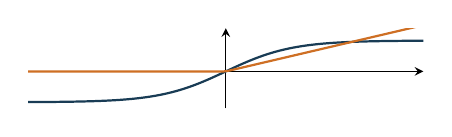
\begin{tikzpicture}
\begin{axis}[axis lines=middle,width=6.6cm,height=2.6cm,xmin=-3,xmax=3,ymin=-1.2,ymax=1.4,xtick=\empty,ytick=\empty,clip=true]
\addplot[domain=-3:3,samples=100,courseBlue,thick]{tanh(x)};
\addplot[domain=-3:3,samples=100,courseOrange,thick]{max(0,x)/2};
\end{axis}
\end{tikzpicture}
\end{center}
\end{frame}

\renewcommand{\slideid}{L2-S42}
\begin{frame}[t]{Forward pass for one input}
\begin{slideitems}
\item For a single scalar input $x$, the forward pass is the sequence
\[
\begin{aligned}
z^{(1)}&=W_1x+b_1, & a^{(1)}&=\sigma(z^{(1)}),\\
z^{(2)}&=W_2a^{(1)}+b_2, & a^{(2)}&=\sigma(z^{(2)}).
\end{aligned}
\]
\[
u_\theta(x)=W_3a^{(2)}+b_3.
\]
\item The intermediate activations are stored because the backward pass reuses them.
\end{slideitems}
\end{frame}

\renewcommand{\slideid}{L2-S43}
\begin{frame}[t]{Forward pass for a batch}
\begin{slideitems}
\item A batch evaluates many inputs at once:
\[
Z^{(1)}=XW_1+\mathbf 1 b_1^\top,
\qquad A^{(1)}=\sigma(Z^{(1)}).
\]
\item The same weights are shared across all rows:
\[
U_\theta(X)=A^{(2)}W_3+\mathbf 1 b_3.
\]
\item Batching changes the computation schedule, not the mathematical function represented by the network.
\end{slideitems}
\end{frame}

\renewcommand{\slideid}{L2-S44}
\begin{frame}[fragile,t]{The loss in PyTorch}
\begin{slideitems}
\item The empirical squared loss is a scalar average over samples:
\[
L_{\rm data}(\theta)=\frac1N\sum_{i=1}^N (u_\theta(x_i)-y_i)^2.
\]
\end{slideitems}
\begin{lstlisting}
prediction = model(train_x)
if prediction.shape != train_y.shape:
    raise ValueError("prediction and target shapes must agree")
loss = ((prediction - train_y)**2).mean()
assert loss.ndim == 0
\end{lstlisting}
\begin{slideitems}
\item Dividing by the parameter count would define a different objective and rescale the gradients.
\end{slideitems}
\end{frame}

\renewcommand{\slideid}{L2-S45}
\begin{frame}[t]{Gradients for the affine baseline}
\begin{slideitems}
\item For $u_{w,b}(x)=wx+b$ and residual $r_i=wx_i+b-y_i$,
\[
L(w,b)=\frac1N\sum_i r_i^2.
\]
\item The derivatives are
\[
\frac{\partial L}{\partial w}=\frac2N\sum_i r_i x_i,
\qquad
\frac{\partial L}{\partial b}=\frac2N\sum_i r_i.
\]
\item Gradient descent replaces the closed-form solve by repeated small parameter updates.
\end{slideitems}
\end{frame}

\renewcommand{\slideid}{L2-S46}
\begin{frame}[t]{Gradient descent as repeated local improvement}
\begin{slideitems}
\item Given a differentiable objective $L(\theta)$, gradient descent uses
\[
\theta_{k+1}=\theta_k-\eta\nabla L(\theta_k).
\]
\item The vector $-\nabla L(\theta_k)$ is the direction of steepest local decrease in Euclidean norm.
\item The scalar $\eta>0$ is the learning rate. It turns a direction into a finite step.
\item The update is local: it uses information at the current point, not a global view of the objective.
\end{slideitems}
\end{frame}

\renewcommand{\slideid}{L2-S47}
\begin{frame}[t]{Gradient descent on a convex quadratic}
\begin{slideitems}
\item For
\[
L(\theta)=\frac12\theta^\top A\theta,
\qquad A=A^\top>0,
\]
the gradient is $\nabla L(\theta)=A\theta$.
\item The update is
\[
\theta_{k+1}=(I-\eta A)\theta_k.
\]
\item The plot shows the iterates moving across level sets toward the minimiser.
\end{slideitems}
\begin{center}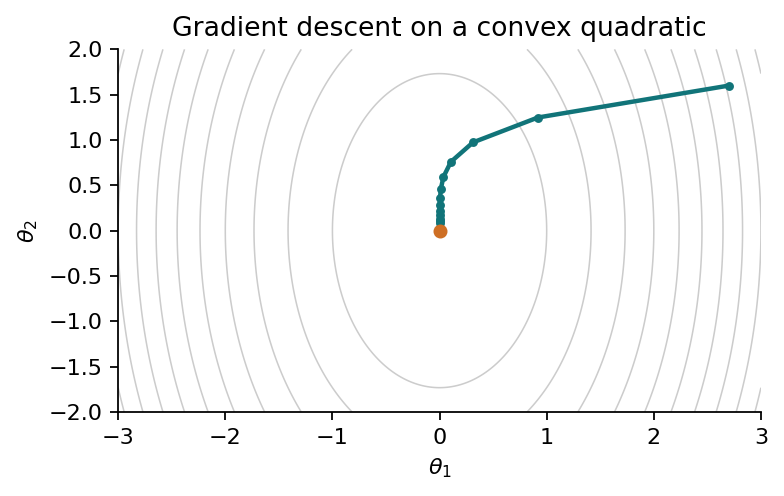
\includegraphics[height=2.75cm]{gd_quadratic_path.png}\end{center}
\end{frame}

\renewcommand{\slideid}{L2-S48}
\begin{frame}[t]{Learning rate: too small, useful, too large}
\begin{slideitems}
\item If $\eta$ is too small, progress is stable but slow.
\item If $\eta$ is in a useful range, the loss decreases quickly.
\item If $\eta$ is too large, updates overshoot the minimiser and may diverge.
\item For the quadratic $L(\theta)=\frac12\theta^\top A\theta$, convergence requires
\[
0<\eta<\frac{2}{\lambda_{\max}(A)}.
\]
\end{slideitems}
\end{frame}

\renewcommand{\slideid}{L2-S49}
\begin{frame}[t]{Learning-rate curves}
\begin{slideitems}
\item A useful diagnostic is the objective value as a function of iteration.
\item The same initial point and the same objective can behave very differently when only $\eta$ changes.
\end{slideitems}
\begin{center}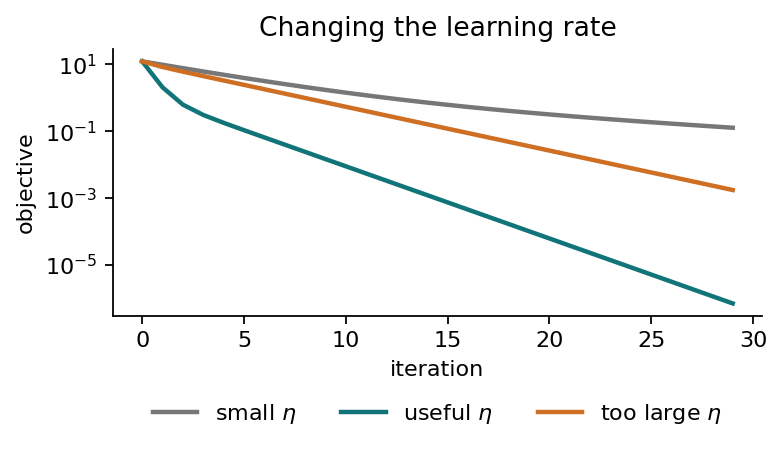
\includegraphics[height=3.15cm]{lr_curves.png}\end{center}
\end{frame}

\renewcommand{\slideid}{L2-S50}
\begin{frame}[t]{Overshooting in one dimension}
\begin{slideitems}
\item On $L(\theta)=\frac12\theta^2$, the update is
\[
\theta_{k+1}=(1-\eta)\theta_k.
\]
\item If $0<\eta<1$, the iterates approach the minimiser without changing sign.
\item If $1<\eta<2$, the iterates oscillate while shrinking.
\item If $\eta>2$, the oscillations grow and the method diverges.
\end{slideitems}
\begin{center}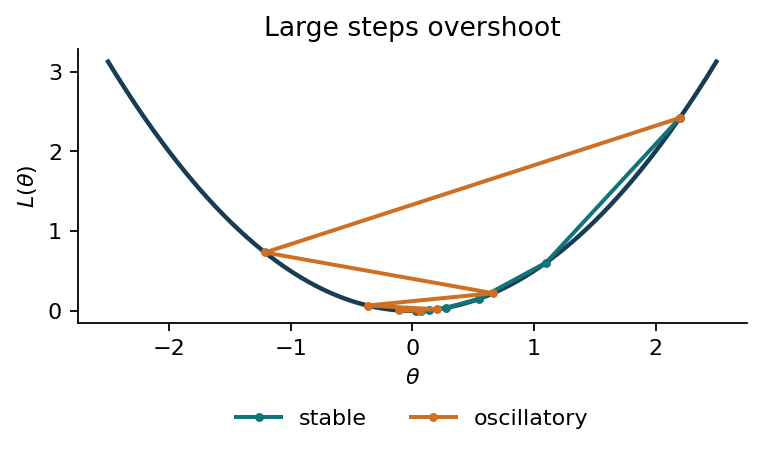
\includegraphics[height=2.75cm]{overshoot.png}\end{center}
\end{frame}

\renewcommand{\slideid}{L2-S51}
\begin{frame}[t]{Non-convex objectives}
\begin{slideitems}
\item Neural-network losses are usually non-convex in $\theta$.
\item Different initialisations can move into different basins of attraction.
\item A small gradient does not necessarily mean that the current point is the best possible predictor.
\end{slideitems}
\begin{center}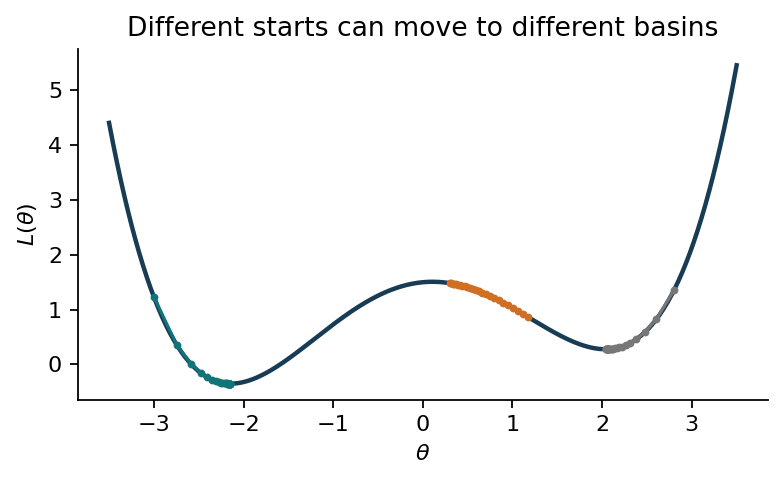
\includegraphics[height=3.0cm]{nonconvex_path.png}\end{center}
\end{frame}

\renewcommand{\slideid}{L2-S52}
\begin{frame}[t]{Local minima, saddle points and flat regions}
\begin{slideitems}
\item A point with $\nabla L(\theta)=0$ is stationary. It may be a local minimum, a local maximum, or a saddle point.
\item In high dimensions, saddle points and flat valleys are common; training can slow down even when no useful minimum has been reached.
\item Permuting hidden units often leaves $u_\theta$ unchanged, so the same function may correspond to many parameter vectors.
\item Repeat training with several seeds to measure sensitivity to initialisation.
\end{slideitems}
\end{frame}

\renewcommand{\slideid}{L2-S53}
\begin{frame}[t]{Stochastic and mini-batch gradient descent}
\begin{slideitems}
\item Full-batch gradient descent uses all samples:
\[
\nabla R_N(\theta)=\frac1N\sum_{i=1}^N \nabla_\theta \ell_i(\theta).
\]
\item Mini-batch SGD uses a subset $B_k$:
\[
g_k=\frac1{|B_k|}\sum_{i\in B_k}\nabla_\theta \ell_i(\theta_k),
\qquad \theta_{k+1}=\theta_k-\eta g_k.
\]
\item The stochastic gradient is noisy but cheaper for large datasets. The noise can also help the iteration leave narrow regions.
\end{slideitems}
\end{frame}

\renewcommand{\slideid}{L2-S54}
\begin{frame}[t]{Projected gradient descent}
\begin{slideitems}
\item If parameters must satisfy a constraint $\theta\in C$, projected GD uses
\[
\theta_{k+1}=\Pi_C\bigl(\theta_k-\eta\nabla L(\theta_k)\bigr).
\]
\item The projection
\[
\Pi_C(z)=\arg\min_{\theta\in C}\|\theta-z\|_2
\]
returns the closest feasible point.
\item This is useful for norm constraints, box constraints, and simple feasibility requirements.
\end{slideitems}
\begin{center}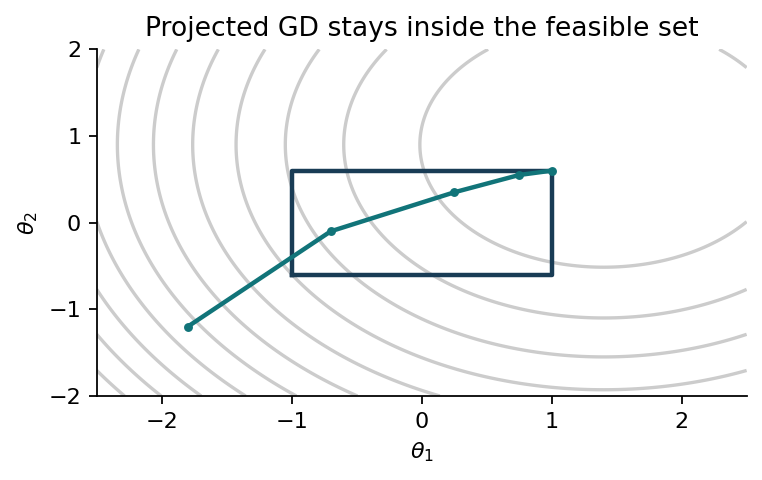
\includegraphics[height=2.65cm]{projected_gd.png}\end{center}
\end{frame}

\renewcommand{\slideid}{L2-S55}
\begin{frame}[t]{Momentum, RMSProp and Adam}
\begin{slideitems}
\item Momentum smooths the update direction:
\[
v_{k+1}=\mu v_k+g_k,
\qquad \theta_{k+1}=\theta_k-\eta v_{k+1}.
\]
\item RMSProp rescales coordinates using a running average of squared gradients.
\item Adam combines momentum and adaptive coordinatewise scaling. It is not plain gradient descent.
\item The optimiser, learning rate, batch size, dtype, seed, and update budget are part of the reported method.
\end{slideitems}
\end{frame}

\renewcommand{\slideid}{L2-S56}
\begin{frame}[fragile,t]{Adam in PyTorch}
\begin{slideitems}
\item Create an Adam optimiser, then use it to update the parameters.
\end{slideitems}
\begin{lstlisting}
optimizer = torch.optim.Adam(
    model.parameters(),
    lr=1e-3,
    weight_decay=0.0,
)
optimizer.zero_grad(set_to_none=True)
loss.backward()
optimizer.step()
\end{lstlisting}
\begin{slideitems}
\item Report Adam and its settings when describing the training run.
\end{slideitems}
\end{frame}

\renewcommand{\slideid}{L2-S57}
\begin{frame}[t]{Backpropagation is the chain rule}
\begin{slideitems}
\item For one neuron,
\[
\begin{aligned}
z&=wx+b, & t&=\tanh z,\\
\widehat y&=at+c, & L&=\frac12(\widehat y-y)^2.
\end{aligned}
\]
\item With $r=\widehat y-y$,
\[
\frac{\partial L}{\partial a}=rt,
\quad
\frac{\partial L}{\partial c}=r,
\quad
\frac{\partial L}{\partial w}=ra(1-t^2)x,
\quad
\frac{\partial L}{\partial b}=ra(1-t^2).
\]
\item Backpropagation applies this chain rule efficiently across the full computational graph.
\end{slideitems}
\end{frame}

\renewcommand{\slideid}{L2-S58}
\begin{frame}[t]{Reverse mode versus forward mode}
\begin{slideitems}
\item If $F:\R^p\to\R^q$, forward mode propagates products $Jv$ and reverse mode propagates products $w^\top J$.
\item Training has many parameters and one scalar loss: $p\gg q=1$, so reverse mode is efficient.
\item Coordinate derivatives of a scalar input are a different request. They differentiate with respect to $x$, not with respect to model parameters.
\item Autograd is exact differentiation of executed operations up to floating-point rounding; it is not a finite-difference approximation.
\end{slideitems}
\end{frame}

\renewcommand{\slideid}{L2-S59}
\begin{frame}[fragile,t]{The five-step training loop}
\begin{slideitems}
\item One full-batch update consists of clearing gradients, evaluating the model, forming the loss, backpropagating, and updating parameters.
\end{slideitems}
\begin{lstlisting}
model.train()
optimizer.zero_grad(set_to_none=True)
prediction = model(train_x)
loss = ((prediction - train_y)**2).mean()
loss.backward()
optimizer.step()
\end{lstlisting}
\begin{slideitems}
\item Alongside this loop, record the loss and check predictions on validation data.
\end{slideitems}
\end{frame}

\renewcommand{\slideid}{L2-S60}
\begin{frame}[fragile,t]{A safer training step}
\begin{slideitems}
\item Add checks that make common failures explicit.
\end{slideitems}
\begin{lstlisting}
prediction = model(train_x)
if prediction.shape != train_y.shape:
    raise ValueError("shape mismatch")
loss = ((prediction - train_y)**2).mean()
if loss.ndim != 0 or not torch.isfinite(loss):
    raise FloatingPointError("invalid loss")
optimizer.zero_grad(set_to_none=True)
loss.backward()
optimizer.step()
\end{lstlisting}
\begin{slideitems}
\item These checks stop training when the shapes or loss are invalid.
\end{slideitems}
\end{frame}

\renewcommand{\slideid}{L2-S61}
\begin{frame}[t]{Regularisation: changing the fitted solution}
\begin{slideitems}
\item Regularisation adds a preference among functions that fit the data similarly well.
\item A common penalised objective is
\[
L_{\rm reg}(\theta)=R_N(\theta)+\lambda\Omega(\theta),\qquad \lambda\ge 0.
\]
\item The penalty $\Omega$ encodes what is considered simple: small weights, sparse weights, smoothness, or another structural bias.
\item Regularisation trades training fit for stability and generalisation.
\end{slideitems}
\end{frame}

\renewcommand{\slideid}{L2-S62}
\begin{frame}[t]{L2 regularisation and weight decay}
\begin{slideitems}
\item L2 regularisation uses
\[
\Omega(\theta)=\frac12\|\theta\|_2^2,
\qquad
L_{\rm reg}=R_N(\theta)+\frac{\lambda}{2}\|\theta\|_2^2.
\]
\item Its gradient adds a shrinkage term:
\[
\nabla L_{\rm reg}=\nabla R_N(\theta)+\lambda\theta.
\]
\item For plain gradient descent,
\[
\theta_{k+1}=(1-\eta\lambda)\theta_k-\eta\nabla R_N(\theta_k).
\]
\item L2 tends to shrink weights smoothly rather than setting them exactly to zero.
\end{slideitems}
\begin{center}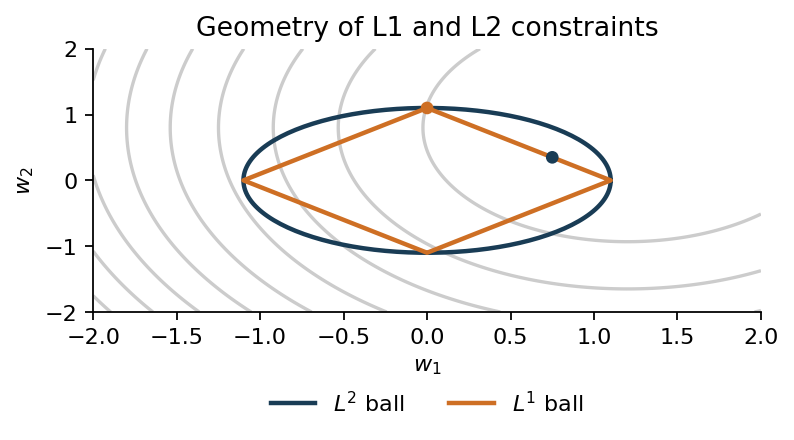
\includegraphics[height=2.25cm]{l1_l2_geometry.png}\end{center}
\end{frame}

\renewcommand{\slideid}{L2-S63}
\begin{frame}[t]{L1 regularisation and sparsity}
\begin{slideitems}
\item L1 regularisation uses
\[
\Omega(\theta)=\|\theta\|_1=\sum_j |\theta_j|.
\]
\item The absolute-value penalty has corners. Those corners make exact zeros common.
\item In the one-dimensional least-squares case, the solution is a soft-thresholding rule:
\[
\widehat\theta_{L1}=\operatorname{sign}(z)\max\{|z|-\lambda,0\}.
\]
\item This is why L1 is associated with feature selection and sparse coefficients.
\end{slideitems}
\begin{center}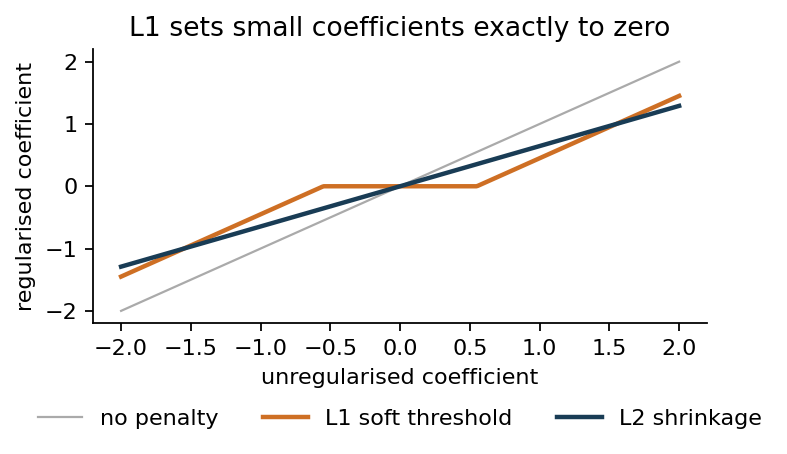
\includegraphics[height=2.25cm]{sparsity_shrinkage.png}\end{center}
\end{frame}

\renewcommand{\slideid}{L2-S64}
\begin{frame}[t]{Elastic net and practical penalties}
\begin{slideitems}
\item Elastic net combines L1 and L2:
\[
L_{\rm reg}(\theta)=R_N(\theta)+\lambda_1\|\theta\|_1+\frac{\lambda_2}{2}\|\theta\|_2^2.
\]
\item L1 encourages sparsity; L2 stabilises and shrinks correlated parameters together.
\item In neural networks, L2 weight decay is common; L1 can be used but may make optimisation less smooth.
\item The penalty strength is a hyperparameter and must be chosen without looking at the test set.
\end{slideitems}
\end{frame}

\renewcommand{\slideid}{L2-S65}
\begin{frame}[t]{Early stopping as implicit regularisation}
\begin{slideitems}
\item Early stopping does not add an explicit penalty to the objective.
\item It restricts the optimisation path by selecting an earlier checkpoint:
\[
\widehat k=\arg\min_k R_{\rm val}(\theta_k).
\]
\item In many problems, late iterations keep reducing training loss while validation loss stops improving.
\item The checkpoint rule must be fixed before the test set is read.
\end{slideitems}
\begin{center}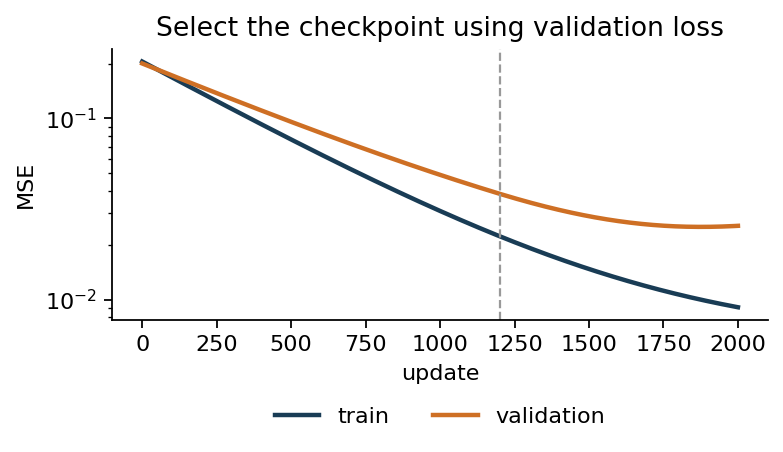
\includegraphics[height=2.75cm]{learning_curves.png}\end{center}
\end{frame}

\renewcommand{\slideid}{L2-S66}
\begin{frame}[t]{Changing width}
\begin{slideitems}
\item Increasing width adds more hidden units per layer:
\[
1\to m\to m\to 1.
\]
\item The parameter count scales approximately like $m^2$ for two hidden layers because the middle matrix has size $m\times m$.
\item Wider networks can fit more complicated functions, but they can also fit noise more easily.
\item Width changes approximation, estimation, and optimisation at the same time; one plot rarely separates the three.
\end{slideitems}
\end{frame}

\renewcommand{\slideid}{L2-S67}
\begin{frame}[t]{Changing depth}
\begin{slideitems}
\item Increasing depth adds more nonlinear compositions:
\[
x\mapsto \sigma(W_L\sigma(\cdots \sigma(W_1x+b_1)\cdots)+b_L).
\]
\item Depth can represent some compositional structures more efficiently than width alone.
\item More depth also changes gradient flow: vanishing gradients, exploding gradients, and sensitivity to initialisation become more relevant.
\item Residual connections and normalisation layers are common practical responses in larger models, but they are not needed for this small regression example.
\end{slideitems}
\end{frame}

\renewcommand{\slideid}{L2-S68}
\begin{frame}[t]{Width and depth in a regression plot}
\begin{slideitems}
\item The plot is schematic: changing architecture changes the set of functions the optimiser can select.
\item Too little capacity underfits; enough capacity can track the signal; excessive flexibility can also track noise.
\end{slideitems}
\begin{center}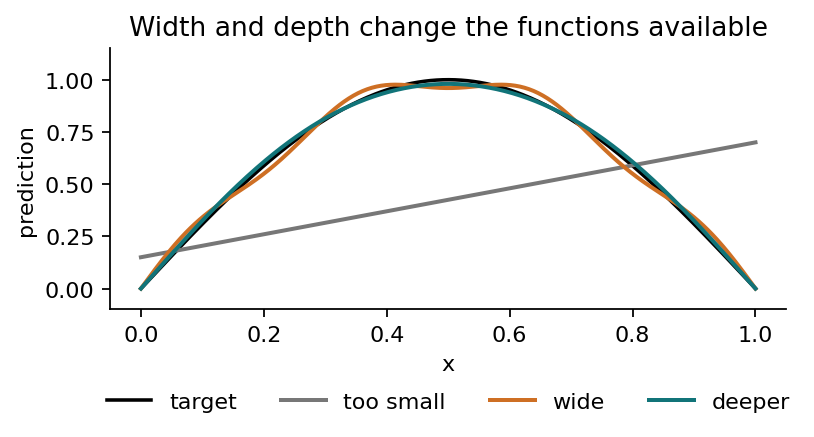
\includegraphics[height=3.15cm]{width_depth_predictions.png}\end{center}
\end{frame}

\renewcommand{\slideid}{L2-S69}
\begin{frame}[t]{Underfitting and overfitting}
\begin{slideitems}
\item Underfitting: the model family is too limited or training has not reached a useful part of it.
\item Overfitting: the model follows sample-specific fluctuations that do not generalise.
\item Both can occur with neural networks; validation data are used to detect the trade-off.
\end{slideitems}
\begin{center}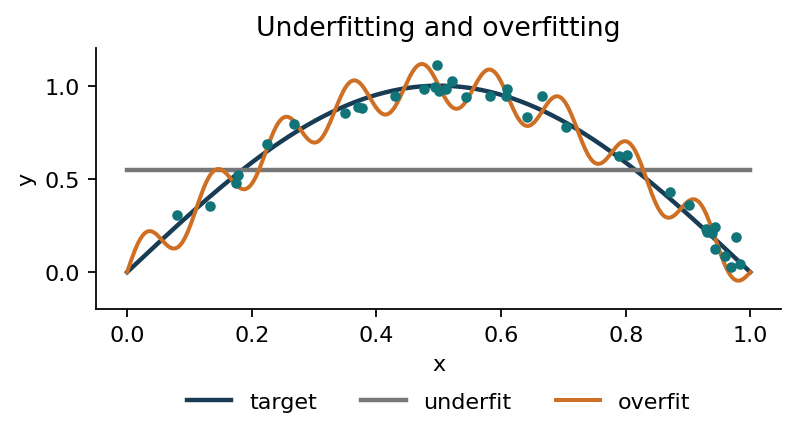
\includegraphics[height=3.0cm]{under_over.png}\end{center}
\end{frame}

\renewcommand{\slideid}{L2-S70}
\begin{frame}[t]{Learning curves and validation}
\begin{slideitems}
\item Training loss measures fit to the data used for gradient updates.
\item Validation loss estimates performance on data not used for updates.
\item A widening gap between the two curves suggests overfitting or an overly long training run.
\end{slideitems}
\begin{center}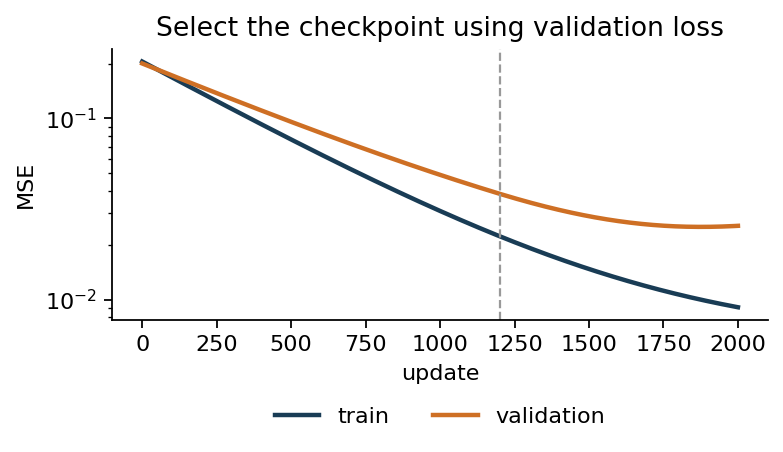
\includegraphics[height=3.0cm]{learning_curves.png}\end{center}
\end{frame}

\renewcommand{\slideid}{L2-S71}
\begin{frame}[fragile,t]{Checkpointing}
\begin{slideitems}
\item Save a copy of the best validation state, not a live reference to changing tensors.
\end{slideitems}
\begin{lstlisting}
model.eval()
with torch.no_grad():
    val_mse = ((model(val_x) - val_y)**2).mean().item()
if val_mse < best_val_mse:
    best_val_mse = val_mse
    best_state = copy.deepcopy(model.state_dict())
    best_step = step
\end{lstlisting}
\begin{slideitems}
\item After training, reload the selected state and evaluate on the test split once.
\end{slideitems}
\end{frame}

\renewcommand{\slideid}{L2-S72}
\begin{frame}[t]{Test evaluation and leakage}
\begin{slideitems}
\item Use the training split for gradient updates.
\item Use the validation split for choices such as width, penalty strength, and selected checkpoint.
\item Use the test split only after these choices are fixed.
\item A number stops being a test estimate as soon as it influences a modelling decision.
\end{slideitems}
\end{frame}

\renewcommand{\slideid}{L2-S73}
\begin{frame}[t]{Metrics: MSE, RMSE and MAE}
\begin{slideitems}
\item Mean squared error is
\[
{\rm MSE}=\frac1M\sum_{j=1}^M(\widehat y_j-y_j)^2.
\]
\item Root mean squared error is
\[
{\rm RMSE}=\sqrt{{\rm MSE}},
\]
which has the same physical units as $y$.
\item Mean absolute error is
\[
{\rm MAE}=\frac1M\sum_{j=1}^M|\widehat y_j-y_j|.
\]
\item Report which metric is being used; they answer related but different questions.
\end{slideitems}
\end{frame}

\renewcommand{\slideid}{L2-S74}
\begin{frame}[fragile,t]{Plotting predictions on a grid}
\begin{columns}[T,totalwidth=\textwidth]
\begin{column}{0.49\textwidth}
\begin{slideitems}
\item A dense grid gives a visual check between observed points.
\end{slideitems}
\begin{lstlisting}
grid = torch.linspace(0, 1, 400,
                      dtype=torch.float64)[:, None]
model.eval()
with torch.no_grad():
    pred = model(grid).cpu().numpy()
\end{lstlisting}
\end{column}
\begin{column}{0.47\textwidth}
\centering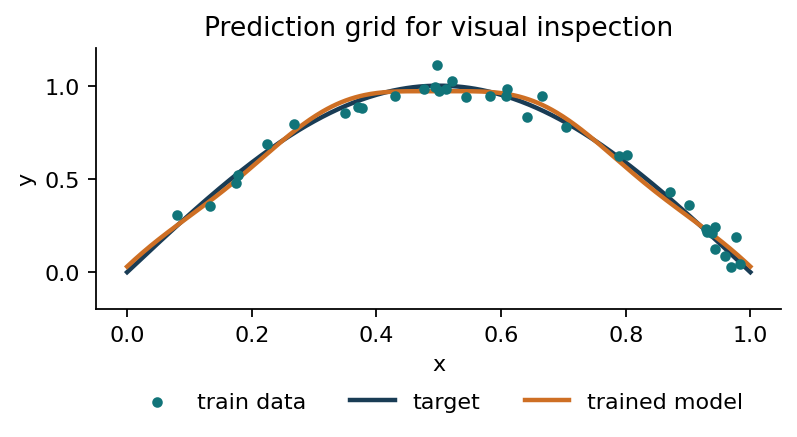
\includegraphics[width=\linewidth]{prediction_grid.png}
\end{column}
\end{columns}
\end{frame}

\renewcommand{\slideid}{L2-S75}
\begin{frame}[t]{Repeated seeds}
\begin{slideitems}
\item Randomness enters through data generation, data splits, initial weights, and sometimes mini-batch order.
\item One seed gives one run; other initialisations can give different results.
\item Repeating seeds helps distinguish systematic behaviour from a lucky or unlucky initialisation.
\item Report mean, spread, and the exact protocol used to generate the runs.
\end{slideitems}
\end{frame}

\renewcommand{\slideid}{L2-S76}
\begin{frame}[t]{Hyperparameter search without leakage}
\begin{slideitems}
\item Hyperparameters include width, depth, learning rate, batch size, penalty strength, optimiser, and training budget.
\item Each candidate is trained on the training set and selected using validation performance.
\item The test set is evaluated only for the selected protocol.
\item If the test set is used to choose a hyperparameter, it becomes part of the selection process.
\end{slideitems}
\end{frame}

\renewcommand{\slideid}{L2-S77}
\begin{frame}[t]{Common implementation bugs}
\begin{slideitems}
\item Shape mismatch: $(N,1)$ compared with $(N,)$ can create an $(N,N)$ residual matrix.
\item Graph break: converting tensors to NumPy inside the loss prevents autograd from computing the required derivative.
\item Gradient accumulation: forgetting \texttt{zero\_grad} adds new gradients to old gradients.
\item Test leakage: selecting the best epoch or architecture by test loss invalidates the final estimate.
\end{slideitems}
\end{frame}

\renewcommand{\slideid}{L2-S78}
\begin{frame}[t]{Formula-to-code dictionary}
\begin{slideitems}
\item Model evaluation:
\[
u_\theta(X)\quad\longleftrightarrow\quad \texttt{model(X)}.
\]
\item Empirical risk:
\[
\frac1N\sum_i(u_\theta(x_i)-y_i)^2
\quad\longleftrightarrow\quad
\texttt{((pred - y)**2).mean()}.
\]
\item Parameter gradient:
\[
\nabla_\theta L(\theta)
\quad\longleftrightarrow\quad
\texttt{loss.backward()}.
\]
\item Parameter update:
\[
\theta\leftarrow\theta-\eta g
\quad\longleftrightarrow\quad
\texttt{optimizer.step()}.
\]
\end{slideitems}
\end{frame}

\renewcommand{\slideid}{L2-S79}
\begin{frame}[t]{A minimal experiment record}
\begin{slideitems}
\item Record the data protocol: target, noise level, sample sizes, and random seeds.
\item Record the model: architecture, activation, parameter count, dtype, and initialisation policy.
\item Record the training protocol: optimiser, learning rate, batch size, penalty, update budget, and checkpoint rule.
\item Record the evaluation protocol: metric, split, and whether the test result was used only once.
\end{slideitems}
\end{frame}

\renewcommand{\slideid}{L2-S80}
\begin{frame}[t]{What to remember}
\begin{slideitems}
\item Supervised regression fits a predictor by minimising a loss on observed data.
\item Gradient descent follows local gradient information; the learning rate, stochasticity, constraints, and optimiser variant change the path.
\item Regularisation changes which fitted functions are preferred: L2 shrinks, L1 promotes sparsity, and early stopping selects along the training path.
\item Choose width and depth using validation data. Report the data, training settings, and test error so others can assess the result.
\end{slideitems}
\end{frame}

\end{document}
